\subsubsection*{Metasploit: Introduction}
\label{subsubsec:Metasploit_Intro}
\addcontentsline{toc}{subsubsection}{Metasploit: Introduction}

\T{Introduction to Metasploit}{
In this and the following modules we will deal with \textbf{Metasploit}, one of the most common and powerful exploitation frameworks in the pentesting environment.\\
Its utility relies on the support it provides throughout the whole exploitation process, from info gathering to post-exploitation.\\

Metasploit has two main versions:
\begin{itemize}
\item Metasploit Pro: the commercial version, providing a GUI and easeness of task automation
\item Metasploit Framework: the open-source version run from the command line
\end{itemize}
Metasploit is composed of three main parts: 
\begin{enumerate}
\item \cd{\textbf{msfconsole}}: this is the main usage interface for the non-commercial version, running as a command-line interface.
\item \textbf{Modules}: supporting modules, e.g pre-made exploits, scanners and payloads.
\item \textbf{Tools}: stand-alone helping tools, moslty for the reconnaissance phase.\\
The most well-known of these are \cd{msfvenom, pattern\_create} and \cd{pattern\_offset}, oh which we will only deal with the first one for the time being.
\end{enumerate}
}
\T{Main Components of Metasploit}{
We launch the Metasploit console by running \cd{msfconsole} on the terminal. \\
Before getting into the actual usage of the different modules and their categories, we clarify some nomenclature about any attack: 
\begin{itemize}
\item Vulnerability: a design, coding or logic flaw affecting the target system. Its exploitation can lead to RCE or the disclosure of confidential information, among others.
\item Exploit: a piece of code taking advantage of a vulnerability in the target system.
\item Payload: code running on the target system to take advantage of the exploit and achieve the attacker's actual goals. 
\end{itemize}
The modules and corresponding categories of Metasploit are divided as follows:
\begin{itemize}
\item \textbf{Auxiliary}: for supporting modules as scanners, crawlers and fuzzers.
\item \textbf{Encoders}: for encoding the exploit and payload hoping that a signature-based antivirus does not catch them.\\
Still, antiviruses work on a database of known threats, comparing incoming files to them and raising an alert if a match is found, so the success of encoders is limited.
\item \textbf{Evasion}: for evading antiviruses and other detection methods.
\item \textbf{Exploits}: as stated above, the code to take advantage of a security flaw in the system. They are organized by target system, e.g android, linux, solaris, windows, etc. . 
\item \textbf{NOPs}: a category of ``waiting modules'' that do nothing (No OPeration), or rather instruct the CPU to do nothing for a complete cycle. They allow for payloads to build up higher sizes.
\item \textbf{Payloads}: as stated above, the code running on the target system to (eventually) further allow to take advantage of the exploitation. They are divided into four categories: \\
	\begin{itemize}
	\item Adapters: wrap single payloads to convert them to different formats, e.g powershell commands.
	\item Singles: self-contained payloads, e.g add a user, launch notepad.exe, etc. that do not need to download an additional component to run.
	\item Stagers: set up a connetion channel between Metasploit and the target system. They usually work in conjunction with staged payloads the following way: the staged payload uploads a stager on the target and then downloads the rest of the payload, called a stage when executed like this.\\
	This allows for smaller initial payloads.
	\item Stages: downloaded by the stager, allows for the use of altogether larger payloads than the small initial payload would allow.
	\end{itemize}
	Metasploit differentiates already in the naming scheme of payloads between single or inline payloads and staged payloads: \\
	an inline payload has an underscore in the name between ``shell'' and ``reverse'', such as \cd{generic/shell\_reverse\_tcp}, whereas a staged payload does not, e.g \cd{windows/x64/shell/reverse\_tcp}
\item \textbf{Post}: used for post-exploitation.

\textbf{NOTE:} to see all available modules of a given category, we run in the msfconsole the command \cd{show <category name>}, e.g \cd{show encoders}
\end{itemize}
\QA{
What is the name of the code taking advantage of a flaw on the target system?
}{
Exploit
}
\QA{
What is the name of the code that runs on the target system to achieve the attacker's goal? 
}{
Payload
}
\QA{
What are self-contained payloads called?
}{
Singles
}
\QA{
Is "windows/x64/pingback\_reverse\_tcp" among singles or staged payload?
}{
Singles
}
}
\T{Msfconsole}{
As instructed before, we call the Metasploit console with the command \cd{msfconsole} on our Terminal.\\
Upon launch, the command line will change to msfX, with X being the version number of Metasploit (at the moment generally 5 or 6).\\
The Metasploit console will support most of the common Linux commands, but not all functionalities of them, such as output redirection. Whereas in the example the execution of a (single, \cd{-c 1} ) ping to Google's 8.8.8.8 IP is shown, I could not reproduce the actual ping nor find it under ``Core Commands'' in the \cd{help}-menu.  \\
To get information on a specific command, we use \cd{help <command>}. To show the command history, we can resort to \cd{history}. Note that the metasploit console supports autocompletion of commands on Tab.\\

The Msfconsole is managed by context, i.e all variables are local unless stated otherwise and will be lost after module change. This is especially relevant for the \cd{RHOSTS} variable, as we usually will want to keep poking at the same address with all our modules.\\

In order to use a given module, we can either run \cd{use <full path to module>} or \cd{use <module-nr-after-search>}, usually with the second variant being shorter despite needing an extra step, namely the number search. We can find the number associated to a Metasploit number at the left of the console output when running a \cd{search} command for the name of the module we'd like to use, e.g \cd{search eternalblue} as in the example. Note that we can perform searches based on number, keywords, target systems, CVEs and more. We then switch to the module calling \cd{use 0} or \cd{use exploit/windows/smb/ms17\_010\_eternalblue}. This way the command prompt changes to the selected module, but we do not enter a different folder, as can be seen by comparison of the output of the \cd{ls} command before and after the module selection. Said module selection only provides a working context we can analyze more deeply via \cd{show options}. This way we can see required and optional arguments, as well as default values for some of them and usage of the module.\\
Depending on the kind of the module we might need e.g a session ID for post-exploitation the connecting modules generate at connection.\\
For the sake of completion, as stated before, we can always run \cd{show} to list available modules in the current context. For general information on the selected context or module we run \cd{info}, or \cd{info <path-to-module>} if we want to access another module and view its related information.\\
To exit a certain module context, run \cd{back}.\\
A last piece of key information related to the \cd{search} command is the rank of the module, based on reliability. Note that this is a general classification and not a completely reliable piece of information to be trusted blindly.\\
A short summary of the ranks can be seen in the following table from the \href{https://github.com/rapid7/metasploit-framework/wiki/Exploit-Ranking}{Metasploit Wiki}:\\
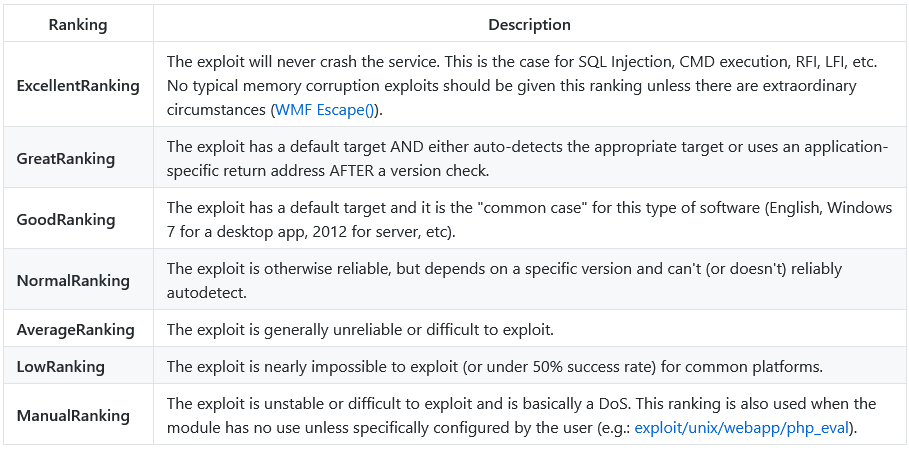
\includegraphics[scale=0.35]{Complete_Beginner_Path/Windows_Exploitation_Basics_Room/Metasploit_Rank_Table.png}\\
\QA{
How would you search for a module related to Apache?
}{
\cd{search Apache}
}
\QA{
Who provided the auxiliary/scanner/ssh/ssh\_login module?
}{
We first run a search on \cd{search ssh\_login} and then \cd{info 0} or conduct a search on the whole path to the given module, wither way seeing it was \cd{``Provided by: \textbf{todb} <todb$@$metasploit.com>}
}
}
\T{Working with modules}{
As stated before, we can (and should) use the \cd{show options} command to know which parameters to set before running any module using the syntax \cd{set <parameter-name> <value>}. After setting these parameters, we can still check them with the \cd{show options} command. \\
The most common parameters to set are: 
\begin{itemize}
\item RHOSTS: stands for remote host, the IP address of the target system. Supports CIDR (Classless Inter-Domain Routing), i.e /24, /16 notation and network ranges ( 10.10.10.xx-10.10.10.yy) as well as files with listed targets, once per line. 
\item RPORT: remote port, the port on the target system upon which the vulnerable, target application runs.
\item PAYLOAD: the payload to be used with the exploit.
\item LHOST: stands for local host, the IP of our attacking machine. 
\item LPORT: local port, the port we will use to establish a reverse shell on.
\item SESSION: as stated before, every connection will have its session ID assigned, and this information will be passed along to the post-exploitation step. 
\end{itemize}
Set values can be overridden by setting a different value to the same parameter, or deleted via \cd{unset <parameter-name>}. Use \cd{unset all} to clear all parameter values.\\

As we stated before, values are stored locally unless set otherwise. This global setting of parameters can be achieved with the command \cd{setg <parameter-value>} (and cleared with \cd{unsetg}).\\

When all module parameters are ready, one launches the module with the \cd{exploit} or \cd{run} command, in combination with the \cd{-z} switch if so desired. This switch will run the exploit and background sessions at the once. The exploits check if the target system is vulnerable to them , but one can check without launching the full exploit with the \cd{check} option if supported.\\

When exploiting a vulnerability, a session is created. If we wish to keep working before taking advanteage of this newly created communication channel, we can send this Meterpreter (more on this later) session to the background with the \cd{background} command, or with the shortcut \cd{Ctrl+Z}.\\
 One can later access all backgrounded sessions with the \cd{sessions} command from the msfconsole or any context console.\\
 To reopen any backgrounded session, we run the command \cd{ sessions -i <session-nr>} using the session ID we learn when running the previous command.\\
 
Last, but not least, it is always important to keep an eye open for the console one is using at each moment: 
On the regular console (\cd{user$@$machine}) one cannot run any Metasploit commands.\\
These are reserved for the msfconsole prompt (\cd{msf6 >} when run without context). This msfconsole can be further specified with context, whose path shows up between ``\cd{msf6}'' and ``\cd{>}'', e.g \cd{msf6 exploit(windows/smb/ms17\_010\_eternalblue) >}. Here one can set local parameters and run the modules. \\
One we get a foothold on the target system, we will have a Meterpreter console (\cd{meterpreter >}) , related to this payload we will later see more about.\\
If we have a shell on the target system, we will see a regular console (see above) but not with our system information but with the data of the target system.\\

\QA{
How would you set the LPORT value to 6666?
}{
\cd{set LPORT 6666}
}
\QA{
How would you set the global value for RHOSTS  to 10.10.19.23 ? 
}{
\cd{setg RHOSTS 10.10.19.23}
}
\QA{
What command would you use to clear a set payload?
}{
\cd{unset payload}
}
\QA{
What command do you use to proceed with the exploitation phase?
}{
\cd{exploit}\\
Note that this is the correct answer ``only'' because of the number of letters of the suggested solution. \cd{run} is an also perfectly valid alias for the same command. 
}

}